\setstretch{1.5}

\clearpage
\subsection{\en{Thread Affinity}}
\emph{\en{Thread Affinity}} είναι η έννοια που περιλαμβάνει την βελτιστοποίηση του χρόνου εκτέλεσης ενός προγράμματος,
μέσω βελτιστοποιήσεων στο εύρος ζώνης μνήμης, την αποφυγή καθυστέρησης μνήμης ή της  καθυστέρησης χρήσης προσωρινής
μνήμης.

To \emph{\en{OpenMP 4.0}} εισάγει ένα σύνολο οδηγιών για την υποστήριξη του \emph{\en{thread
affinity}}\cite{thread_affinity}. Η πλειοψηφία πλέον των μηχανημάτων βασίζονται στην \emph{\en{cc-NUMA}} αρχιτεκτονική.
Η \emph{\en{cc-NUMA}} αρχιτεκτονική συντίθεται από δυο ειδικότερες έννοιες:
\begin{itemize}
\item{
\textbf{Συνοχή Μνήμης(\en{Cache Coherence)}}: Στη σύγχρονα πολυπύρηνα συστήματα, σε κάθε πυρήνα εννοείται η ύπαρξη μνήμης \en{Cache} που έχει ως στόχο τη μείωση της κυκλοφορίας στο δίαυλο μνήμης. Ο όρος συνοχή σημαίνει οτι όταν ένας επεξεργαστής ενημερώνει μια θέση της κρυφής μτου μνήμης, τότε όλοι οι άλλοι επεξεργαστές και η κύρια μνήμη, ενημερώνονται έγκαιρα για την τροποποίηση αυτή\cite{pdblab}.
}

\item{
\textbf{\en{NUMA - Non Uniform Memory Access}}: Σε ένα πολυπύρηνο σύστημα επεξεργαστών, ένας επεξεργαστής έχει τη δυνατότητα προσπέλασης της μνήμης του άλλου, αλλά ο απαιτούμενος χρόνος προσπέλασής της δεν είναι ίσος με αυτό της τοπικής του μνήμης\cite{pdplab}. 
}
\end{itemize}



Ο λόγος που κυριάρχησε το σύστημα μνήμης, είναι η συνεχής αύξηση του αριθμού των επεξεργαστών. Η μονολιθική
διασύνδεση μνήμης με σταθερό εύρος ζώνης μνήμης θα αποτελούσε πρόβλημα στην ραγδαία αύξηση των επεξεργαστών.

Στη \emph{\en{cc-NUMA}} αρχιτεκτονική κάθε υποδοχή συνδέεται με ένα υποσύνολο της συνολικής μνήμης του συστήματος. Μία
διασύνδεση ενώνει τα υποσύνολα μεταξύ τους και δημιουργεί την εικόνα ενιαίας μνήμης στον χρήστη. Ένα τέτοιο σύστημα
είναι ευκολότερο να επεκταθεί.

Το πλεονέκτημα της διασύνδεσης είναι ότι η εφαρμογή έχει πρόσβαση σε όλη την μνήμη του συστήματος, ανεξάρτητα από το που
βρίσκονται τα δεδομένα. Ωστόσο, πλέον ο χρόνος πρόσβασης σε αυτά δεν είναι σταθερός καθώς εξαρτάται από τη θέση τους
στη μνήμη.

\clearpage

\begin{figure}[h]
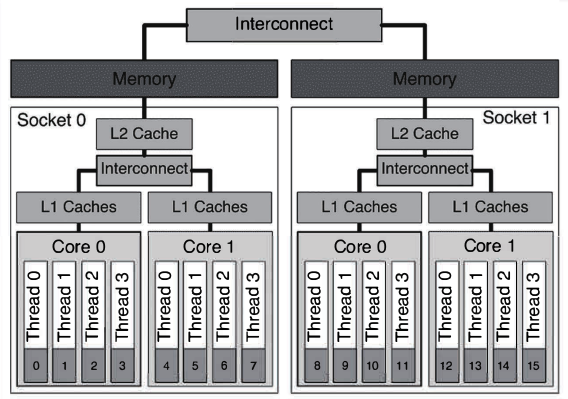
\includegraphics[width=1\textwidth]{numa}
\centering
\captionsetup{justification=centering, singlelinecheck=false}
	\caption{Αρχιτεκτονική \en{cc-NUMA}\cite{thenextstep152}}
\label{fig:numa}
\end{figure}

\subsubsection{\emph{\en{Thread affinity}} στο \emph{\en{OpenMP 4.0}}}
\mbox{}
Με το \emph{\en{thread affinity}} μπορεί να αποτραπεί η μετάβαση μιας διαδικασίας \emph{\en{MPI}} ή ενός νήματος του
\emph{\en{OpenMP}} σε απομακρυσμένο υλικό. Η μετάβαση αυτή θα μπορούσε να προκαλέσει μείωση της απόδοσης του
προγράμματος. Η έκδοση 4.0 του \emph{\en{OpenMP}} εισήγαγε ρυθμίσεις για το χειρισμό του \emph{\en{affinity}} μέσω των
μεταβλητών περιβάλλοντος  \emph{\en{OMP\_PLACES}} και \emph{\en{OMP\_PROC\_BIND}}\cite{affinity1}. \ \\
\clearpage
\paragraph{\emph{\en{Thread Binding}}}
\ \\
Οι προαναφερθείσες μεταβλητές, μπορούν να καθορίσουν σε ποια θέση στο υλικό θα ανατεθούν τα νήματα μια ομάδας που
δημιουργήθηκε για να εκτελέσει μια εργασία. \ \\
\textbf{Παράδειγμα}: Αν υπάρχουν δύο \emph{\en{sockets}} και ορισθεί $$OMP\_PLACES=sockets$$ τότε:
\setlist[1]{itemsep=-10pt}
\begin{itemize}
\item{το νήμα 0 θα πάει στο \emph{\en{socket} 0}}
\item{το νήμα 1 θα πάει στο \emph{\en{socket} 1}}
\item{το νήμα 2 θα πάει στο \emph{\en{socket} 0}} κοκ.
\end{itemize}

Επίσης, αν δυο \emph{\en{socket}} έχουν συνολικά 16 πυρήνες και ο χρήστης ορίσει $$OMP\_PLACES=cores$$
\begin{center}και\end{center} $$OMP\_PROC\_BIND=close$$ 

τότε:
\begin{itemize}
\item{το νήμα 0	θα πάει στον πυρήνα 0 που βρίσκεται στο \emph{\en{socket}} 0}
\item{το νήμα 1	θα πάει στον πυρήνα 1 που βρίσκεται στο \emph{\en{socket}} 0}
\item{το νήμα 2	θα πάει στον πυρήνα 2 που βρίσκεται στο \emph{\en{socket}} 0}
\item{...}
\item{το νήμα 7 στον πυρήνα 7 του \emph{\en{socket}} 0}
\item{το νήμα 8 στον πυρήνα 8 του \emph{\en{socket}} 1, κλπ}
\end{itemize}

Η μεταβλητή \emph{\en{OMP\_PROC\_BIND}} καθορίζει τον τρόπο με τον οποίο τα νήματα ανατίθενται στους πόρους. Η επιλογή
\emph{\en{OMP\_PROC\_BIND = close}} σημαίνει ότι η ανάθεση περνά διαδοχικά στις διαθέσιμες θέσεις. Μια άλλη αποδεκτή
τιμή για το \emph{\en{OMP\_PROC\_BIND}} είναι η \emph{\en{spread}}. Η λειτουργία της φαίνεται στο παρακάτω παράδειγμα: 

\clearpage
\textbf{Παράδειγμα}, για:
$$OMP\_PLACES=cores$$
$$OMP\_PROC\_BIND=spread$$

\begin{itemize}
\item{το νήμα 0 πάει στον πυρήνα 0, που βρίσκεται στο \emph{\en{socket}} 0}
\item{το νήμα 1 πάει στον πυρήνα 8, που βρίσκεται στο \emph{\en{socket}} 1}
\item{το νήμα 2 πάει στον πυρήνα 1, που βρίσκεται στο \emph{\en{socket}} 0}
\item{...}
\item{το νήμα 15 πάει στον πυρήνα 15, που βρίσκεται στο \emph{\en{socket}} 1}
\end{itemize}

Η επιλογή \emph{\en{OMP\_PROC\_BIND = master}} αναθέτει τα νήματα στο ίδιο σημείο που είναι και το κύριο νήμα της ομάδας.
Αυτή η επιλογή χρησιμοποιείται όταν δημιουργούνται πολλές ομάδες αναδρομικά.

Εκτός από τις επιλογές \emph{\en{cores}} και \emph{\en{sockets}} για τη μεταβλητή \emph{\en{OMP\_PLACES}}, υπάρχει και η
\emph{\en{threads}} που χρησιμοποιείται σε ειδικές περιπτώσεις αρχιτεκτονικής, δηλαδή σε περιπτώσεις που οι επεξεργαστές
περιέχουν νήματα\en{(hardware threads)}\cite{affinity2}.

Το παράδειγμα που ακολουθεί, επιβεβαιώνει την προαναφερθείσα θεωρία. Στην παρακάτω ρουτίνα, κάθε νήμα αναλαμβάνει να εκτυπώσει ενα μήνυμα. Το μήνυμα αναφέρει σε ποιον πυρήνα ανήκει το νήμα αυτό\cite{klencockwood}.
\selectlanguage{english}
\begin{spacing}{1.0}
\begin{lstlisting}[language=C++, caption={\el{Παράδειγμα} \en{Affinity}} , frame=tb]{Name}
int main( int argc, char**argv )
{
#pragma omp parallel
    {
#pragma omp critical
        std::cout << "Running from thread " <<
            omp_get_thread_num() + 1 <<
            " of " << omp_get_num_threads() <<
            " on cpu " << sched_getcpu() <<
            std::endl;
     }
     return 0;
 }

\end{lstlisting}
\end{spacing}
\selectlanguage{greek}

\clearpage
\selectlanguage{english}
\begin{spacing}{1.0}
\begin{lstlisting}[language=C++, caption={Affinity: \el{Αποτελέσματα εκτέλεσης}} , frame=tb]{Name}
Running from thread 15 of 16 on cpu 12
Running from thread 3  of 16 on cpu 11
Running from thread 1  of 16 on cpu 15
Running from thread 6  of 16 on cpu 8
Running from thread 12 of 16 on cpu 10
Running from thread 9  of 16 on cpu 9
Running from thread 8  of 16 on cpu 6
Running from thread 14 of 16 on cpu 14
Running from thread 2  of 16 on cpu 3
Running from thread 7  of 16 on cpu 0
Running from thread 10 of 16 on cpu 1
Running from thread 13 of 16 on cpu 2
Running from thread 16 of 16 on cpu 13
Running from thread 11 of 16 on cpu 7
Running from thread 5  of 16 on cpu 5
Running from thread 4  of 16 on cpu 4

\end{lstlisting}
\end{spacing}
\selectlanguage{greek}
\ \\
\ \\
Εκτελώντας το ίδιο πρόβλημα αφού πρώτα χρησιμοποιηθεί η εντολή $OMP\_PLACES="\{0\}"$ τα αποτελέσματα δείχνουν ότι όλα τα νήματα δημιουργούνται απο τον πυρήνα με \en{id} 0:

\selectlanguage{english}
\begin{spacing}{1.0}
\begin{lstlisting}[language=C++, caption={Affinity: \el{Αποτελέσματα εκτέλεσης} $OMP\_PLACES="\{0\}"$} , frame=tb]{Name}
Running from thread 1  of 16 on cpu 0
Running from thread 10 of 16 on cpu 0
Running from thread 11 of 16 on cpu 0
Running from thread 12 of 16 on cpu 0
Running from thread 13 of 16 on cpu 0
Running from thread 14 of 16 on cpu 0
Running from thread 7  of 16 on cpu 0
Running from thread 15 of 16 on cpu 0
Running from thread 16 of 16 on cpu 0
Running from thread 6  of 16 on cpu 0
Running from thread 8  of 16 on cpu 0
Running from thread 5  of 16 on cpu 0
Running from thread 9  of 16 on cpu 0
Running from thread 4  of 16 on cpu 0
Running from thread 3  of 16 on cpu 0
Running from thread 2  of 16 on cpu 0

\end{lstlisting}
\end{spacing}
\selectlanguage{greek}
\clearpage
Αντίστοιχα, με χρήση της $OMP\_PLACES="\{0:4\}"$, τα αποτελέσματα είναι τα παρακάτω:

\selectlanguage{english}
\begin{spacing}{1.0}
\begin{lstlisting}[language=C++, caption={Affinity: \el{Αποτελέσματα εκτέλεσης} $OMP\_PLACES="\{0:4\}"$} , frame=tb]{Name}
Running from thread 15 of 16 on cpu 0
Running from thread 12 of 16 on cpu 1
Running from thread 2  of 16 on cpu 2
Running from thread 4  of 16 on cpu 3
Running from thread 13 of 16 on cpu 1
Running from thread 1  of 16 on cpu 0
Running from thread 3  of 16 on cpu 2
Running from thread 11 of 16 on cpu 3
Running from thread 14 of 16 on cpu 1
Running from thread 6  of 16 on cpu 2
Running from thread 9  of 16 on cpu 3
Running from thread 16 of 16 on cpu 1
Running from thread 7  of 16 on cpu 2
Running from thread 10 of 16 on cpu 3
Running from thread 8  of 16 on cpu 0
Running from thread 5  of 16 on cpu 1

\end{lstlisting}
\end{spacing}
\selectlanguage{greek}

Επίσης, στο παράδειγμα που ακολουθεί, η οδηγία \en{OMP\_PROC\_BIND} είναι υπεύθυνη για τη δημιουργία όλων των νημάτων στον ίδιο πυρήνα με το κύριο νήμα:

\selectlanguage{english}
\begin{spacing}{1.0}
\begin{lstlisting}[language=C++, caption={\el{Παράδειγμα} \en{Affinity}} , frame=tb]{Name}
int main( int argc, char**argv )
 {
     for (int i=1; i<100; i++){
     #pragma omp parallel
         {
             printf( "Running from thread %d of %d on cpu %2d!\n",
                 omp_get_thread_num()+1,
                 omp_get_num_threads(),
                 sched_getcpu());
         }
     }
     return 0;
 }

\end{lstlisting}
\end{spacing}
\selectlanguage{greek}
\ \\

οπου για $OMP\_PROC\_BIND="master"$, τα αποτελέσματα που εκτυπώνονται είναι τα εξής:
\ \\
\selectlanguage{english}
\begin{spacing}{0.8}
\begin{lstlisting}[language=C++, caption={Affinity: \el{Αποτελέσματα εκτέλεσης} $OMP\_PROC\_BIND="master"$ } , frame=tb]{Name}
Running from thread 1  of 16 on cpu  0!
Running from thread 7  of 16 on cpu  0!
Running from thread 11 of 16 on cpu  0!
Running from thread 10 of 16 on cpu  0!
Running from thread 12 of 16 on cpu  0!
Running from thread 13 of 16 on cpu  0!
Running from thread 14 of 16 on cpu  0!
Running from thread 15 of 16 on cpu  0!
Running from thread 16 of 16 on cpu  0!
Running from thread 8  of 16 on cpu  0!
...
Running from thread 2  of 16 on cpu  0!
Running from thread 1  of 16 on cpu  0!
Running from thread 7  of 16 on cpu  0!
Running from thread 11 of 16 on cpu  0!
Running from thread 10 of 16 on cpu  0!
Running from thread 12 of 16 on cpu  0!
Running from thread 13 of 16 on cpu  0!
Running from thread 14 of 16 on cpu  0!
Running from thread 15 of 16 on cpu  0!
Running from thread 16 of 16 on cpu  0!
Running from thread 8  of 16 on cpu  0!
Running from thread 9  of 16 on cpu  0!

\end{lstlisting}
\end{spacing}
\selectlanguage{greek}


Αξίζει τέλος να σημειωθεί η χρήση του προγράμματος \en{numactl}, που έχει ως στόχο τον έλεγχο της πολιτικής διεργασιών και διαχείριση της κοινόχρηστης μνήμης. Στο μηχάνημα εκτέλεσης των προγραμμάτων η εντολή \en{\emph{numactl -H}} δίνει τα παρακάτω αποτελέσματα:

\selectlanguage{english}
\begin{spacing}{0.8}
\begin{lstlisting}[language=C++, caption={\el{Αποτελέσματα} \en{numactl -H}} , frame=tb]{Name}
available: 4 nodes (0-3)
node 0 cpus: 0 1 2 3
node 0 size: 3944 MB
node 0 free: 2660 MB
node 1 cpus: 4 5 6 7
node 1 size: 4030 MB
node 1 free: 1863 MB
node 2 cpus: 12 13 14 15
node 2 size: 4030 MB
node 2 free: 2655 MB
node 3 cpus: 8 9 10 11
node 3 size: 4030 MB
node 3 free: 2105 MB
node distances:
node   0   1   2   3
  0:  10  16  16  16
  1:  16  10  16  16
  2:  16  16  10  16
  3:  16  16  16  10
\end{lstlisting}
\end{spacing}
\selectlanguage{greek}


\subsubsection{Το \emph{\en{thread affinity}} στην πράξη}
Δυστυχώς, δεν υπάρχει ιδανική επιλογή για τη ρύθμιση της τοποθέτησης νήματος και της συγγένειας. Η επιλογή
εξαρτάται από την εκάστοτε εφαρμογή που πρόκειται να εκτελεστεί. Ακόμη, ο χρήστης θα πρέπει να λαμβάνει υπόψη τις εξής
παραμέτρους\cite{affinity3}:
\begin{itemize}
\item{Ο χρόνος εκτέλεσης ενός προγράμματος μπορεί να επηρεαστεί από άλλες εργασίες που εκτελούνται στο ίδιο μηχάνημα εκείνη τη στιγμή και μοιράζονται πρόσβαση στο δίκτυο, τον δίαυλο μνήμης και στην προσωρινή μνήμη.}
\item{Το λειτουργικό σύστημα του μηχανήματος εκτελεί ταυτόχρονα τις δικές του εργασίες}
\end{itemize}

